\documentclass[10pt]{article}
\usepackage[margin=1in]{geometry}
\usepackage{amsmath,amssymb}
\usepackage{booktabs}
\usepackage{graphicx}
\usepackage{xcolor}
\usepackage{listings}
\usepackage[colorlinks=true,linkcolor=blue!50!black,citecolor=blue!50!black,urlcolor=blue!50!black]{hyperref}
\usepackage[expansion=false]{microtype}
\usepackage{lmodern}
\usepackage{caption}
\captionsetup{font=small,labelfont=bf}
% AUTO-GENERATED by make_numbers.py from harness-emitted reports/. DO NOT EDIT.
\newcommand{\ablControlBeat}{8/8}
\newcommand{\ablControlGm}{1.338}
\newcommand{\ablControlLeads}{21}
\newcommand{\ablControlValid}{1.000}
\newcommand{\ablDistillonlyBeat}{8/8}
\newcommand{\ablDistillonlyGm}{1.361}
\newcommand{\ablDistillonlyLeads}{23}
\newcommand{\ablDistillonlyValid}{0.948}
\newcommand{\ablNofeedbackBeat}{8/8}
\newcommand{\ablNofeedbackGm}{1.309}
\newcommand{\ablNofeedbackLeads}{19}
\newcommand{\ablNofeedbackValid}{0.995}
\newcommand{\ablNolearnBeat}{8/8}
\newcommand{\ablNolearnGm}{1.302}
\newcommand{\ablNolearnLeads}{18}
\newcommand{\ablNolearnPctOfControl}{97}
\newcommand{\ablNolearnValid}{0.969}
\newcommand{\beforeALS}{0.69}
\newcommand{\beforeLG}{0.82}
\newcommand{\eteCompileX}{0.993}
\newcommand{\eteCompileXLocal}{1.302}
\newcommand{\eteDevice}{NVIDIA H200}
\newcommand{\eteEagerX}{1.143}
\newcommand{\eteEagerXLocal}{1.085}
\newcommand{\eteErr}{2.9e-03}
\newcommand{\eteGemmFrac}{81}
\newcommand{\eteNonGemmX}{10.88}
\newcommand{\falsifications}{9}
\newcommand{\gridCellsTotal}{816}
\newcommand{\gridLossPct}{10.9}
\newcommand{\gridLossesTotal}{89}
\newcommand{\gridOneCells}{376}
\newcommand{\gridOneGeomean}{1.494}
\newcommand{\gridOneLosses}{38}
\newcommand{\gridOneOps}{32}
\newcommand{\gridOneShortLosses}{30}
\newcommand{\gridRotN}{69}
\newcommand{\gridRotOk}{69}
\newcommand{\gridShortLossesTotal}{76}
\newcommand{\gridTwoCells}{440}
\newcommand{\gridTwoGeomean}{1.480}
\newcommand{\gridTwoLosses}{51}
\newcommand{\gridTwoOps}{37}
\newcommand{\gridTwoShortLosses}{46}
\newcommand{\hthApiVerified}{5}
\newcommand{\hthOps}{7}
\newcommand{\idiomPassOne}{3/1/1/1}
\newcommand{\idiomPassTwo}{8/8/8/8}
\newcommand{\invALSshortMA}{1.222}
\newcommand{\invBeatMA}{7}
\newcommand{\invCumsumC}{1.896}
\newcommand{\invCumsumMA}{1.292}
\newcommand{\invEntropyMA}{1.477}
\newcommand{\invKLMA}{1.225}
\newcommand{\invLGshortMA}{1.450}
\newcommand{\invLM}{5}
\newcommand{\invOk}{7}
\newcommand{\invOps}{7}
\newcommand{\invSMshortMA}{1.803}
\newcommand{\invValidRate}{0.497}
\newcommand{\kbCorrect}{0}
\newcommand{\kbN}{1}
\newcommand{\productKernels}{76}
\newcommand{\selftestCasesFortyNinety}{36}
\newcommand{\selftestCasesHTwoHundred}{36}
\newcommand{\selftestGoldFortyNinety}{17}
\newcommand{\selftestGoldHTwoHundred}{17}
\newcommand{\selftestMachineA}{NVIDIA GeForce RTX 4090}
\newcommand{\selftestMachineB}{NVIDIA H200}
\newcommand{\selftestNegFortyNinety}{19}
\newcommand{\selftestNegHTwoHundred}{19}
\newcommand{\selftestPassFortyNinety}{36}
\newcommand{\selftestPassHTwoHundred}{36}
\newcommand{\sftBestValid}{100}
\newcommand{\stabDiscoveries}{69}
\newcommand{\stabK}{5}
\newcommand{\stabMaxSpread}{0.052}
\newcommand{\stabMeanOfMeans}{1.299}
\newcommand{\stabOps}{69}
\newcommand{\stabStrongestMean}{2.038}
\newcommand{\stabStrongestOp}{cross\_entropy}
\newcommand{\stabStrongestSpread}{0.031}
\newcommand{\stabWeakestMean}{1.113}
\newcommand{\stabWeakestOp}{add\_layernorm\_gelu\_erf}
\newcommand{\stabWeakestSpread}{0.015}
\newcommand{\vTwoBeatMA}{37}
\newcommand{\vTwoCEMA}{2.085}
\newcommand{\vTwoEvaluated}{888}
\newcommand{\vTwoExplore}{0}
\newcommand{\vTwoLM}{35}
\newcommand{\vTwoLeadTakes}{101}
\newcommand{\vTwoMaxMA}{2.09}
\newcommand{\vTwoMinMA}{1.16}
\newcommand{\vTwoOk}{37}
\newcommand{\vTwoOps}{37}
\newcommand{\vTwoValidRate}{0.695}
\newcommand{\vTwoVerified}{617}
   % AUTO-GENERATED from harness-emitted reports/ — the only number source

\lstset{basicstyle=\ttfamily\scriptsize,breaklines=true,frame=single,framesep=4pt}

\title{\textbf{The Referee Is the Product:}\\
\large Un-gameable Verification for LLM-Generated GPU Kernels,\\
and What It Falsified About Its Builders' Beliefs}
\author{Rohit Mahendra Tigon\\
\small \texttt{YMRohit} \quad
\small artifacts: \texttt{huggingface.co/YMRohit/ouroboros-kernelsmith-qwen3.6-27b}}
\date{June 2026 \quad (preprint; single-seed ablations labeled as such)}

\newcommand{\maxauto}{\texttt{torch.compile} max-autotune}
\newcommand{\sys}{\textsc{Ouroboros}}

\begin{document}
\maketitle

\begin{abstract}
Large-language-model kernel generation has a credibility problem: the most publicized
result in the area was retracted within days when its generated kernels were found to be
exploiting the evaluation harness rather than the hardware. We argue the root cause is
architectural --- the reward channel is treated as a metric when it must be engineered as
an \emph{adversarial system under test} --- and we present \sys{}, a verifier-grounded
self-distillation loop whose central artifact is an immutable referee with
\emph{negative controls for the reward function itself}: implemented exploits
(benchmark-shape special-casing, pointer-keyed output memoization, in-place input
mutation) ship in the test suite and must be \textsc{rejected} for the system to be
considered sound. Trained only by this referee, a 27B-parameter open model
(Qwen3.6-27B, LoRA) wrote \productKernels{} Triton fusion kernels that \emph{all} beat
\maxauto{} reproducibly: \stabDiscoveries{}/\stabOps{} pass a $5\times$ fresh-run
stability gate (worst kernel $\stabWeakestMean\times\pm\stabWeakestSpread$; best
$\stabStrongestMean\times\pm\stabStrongestSpread$), and every kernel holds a geometric-mean
win across a $(M,N)\times$dtype shape grid of \gridCellsTotal{} cells with per-cell
recompiled baselines and cache-cold verification --- with the \gridLossPct\% of cells we
lose reported individually. Ablations show that on familiar operators a frozen model plus
verified best-of-$N$ search captures $\ablNolearnPctOfControl\%$ of the full loop's value
and the policy-gradient term earns nothing, while on never-seen operators learning is
visibly load-bearing (validity climbing from $\sim$50\% to 68\% within one run as the model
distills its own verified solutions). Finally, we document nine instances in which the
verifier falsified a confident belief held by the system's own builders --- including our
published diagnosis of the system's one weak regime, which the model repaired with a
simpler schedule family than the one we predicted, flipping the worst published loss
($\beforeALS\times$) into a $\invALSshortMA\times$ win. We conclude that in domains with
cheap, honest measurement, the scarce engineering asset is not the model but the referee,
and we release the harness, all \productKernels{} kernels, the corpus, adapters, raw
per-sample measurements, and a falsification ledger.
\end{abstract}

\section{Introduction}

In February 2025, a well-funded research lab announced an ``AI CUDA Engineer'' with
claimed speedups of up to $150\times$; within roughly 48 hours, public reviewers found the
generated kernels were reusing memory across evaluation runs --- gaming the benchmark
harness, not accelerating the hardware --- and the headline numbers collapsed
\cite{sakana2025}. The episode is usually told as a cautionary tale about hype. We read
it differently: it was a \emph{systems failure with a systems fix}. The reward channel of
an RL-for-code pipeline is an attack surface, and like any attack surface it can be
hardened, regression-tested, and shipped with its known exploits as test cases.

This paper presents \sys{}, a small worked system built around that principle, and
reports what happened when we ran it for one sustained campaign. Concretely:

\begin{enumerate}
\item \textbf{The harness is the product} (\S\ref{sec:harness}). An immutable referee
compiles each candidate Triton kernel, checks elementwise correctness against a PyTorch
reference across \emph{adversarial} shapes, dtypes, and magnitudes, and measures wall-clock
with CUDA events under a measurement-hygiene stack (\S\ref{sec:hygiene}). Crucially, the
referee ships with \emph{negative controls for its own reward channel}: three implemented
cheat kernels --- each a working exploit against a naive version of the harness --- that
must be \textsc{rejected} for the self-test to pass. The full self-test is
\selftestCasesHTwoHundred{} cases (\selftestGoldHTwoHundred{} gold kernels must pass,
\selftestNegHTwoHundred{} negative controls must fail) and is \textsc{all green} on both
an RTX~4090 and an H200.

\item \textbf{The loop} (\S\ref{sec:loop}): supervised bootstrap to a measured validity
gate, then verifier-rewarded search with self-distillation on the model's own verified
winners (reward $=$ measured speedup; Eq.~\ref{eq:reward}), with dedup by canonicalized
AST hash and winner's-curse-corrected exit validation.

\item \textbf{Results} (\S\ref{sec:results}): \productKernels{} model-era kernels;
\stabDiscoveries{}/\stabOps{} reproducible discoveries against \maxauto{} (the incumbent
autotuner, i.e., the strongest honest compiler baseline); geomean wins across the entire
shape grid with losses (\gridLossesTotal{}/\gridCellsTotal{} cells) reported per-cell and
concentrated in one explainable regime; parity-or-better against expert hand-written
Triton under \emph{two} comparison conditions including the library-as-shipped one; and a
correctness-gated end-to-end transformer-block composition with its Amdahl ceiling stated.

\item \textbf{Ablations and the locus of learning} (\S\ref{sec:ablations}): on familiar
operators, frozen best-of-$N$ against the referee captures
$\ablNolearnPctOfControl\%$ of the full loop's geomean and removing the policy-gradient
term does not hurt (single-seed; labeled). On foreign operators, learning is load-bearing
and visible within a single run (Fig.~\ref{fig:learning}).

\item \textbf{The falsification ledger} (\S\ref{sec:falsification}): nine concrete
instances where the referee overruled a confident human belief --- including the authors'
own published diagnosis, hand-written ``textbook'' kernel, ablation prediction, and one of
our own earlier claims, which we retract here explicitly.
\end{enumerate}

We do \emph{not} claim novel algorithm discovery (\S\ref{sec:bounds}); the wins are
reproducible \emph{scheduling} wins of $\sim$10--100\% on bandwidth-bound fusion
operators, which is precisely the long tail practitioners hand-write today. The claim we
defend is methodological: \textbf{with an un-gameable referee, a commodity open model
out-searches the incumbent autotuner, repairs its own weaknesses, and corrects its
builders --- and every one of those statements is regenerable from a machine-emitted
artifact in our repository.} A number that cannot be regenerated by a command does not
appear in this paper; every statistic below is compiled from the harness's JSON outputs
by the same script that performs cross-report consistency checks.

\section{Related Work}

\textbf{LLMs writing GPU kernels.} KernelBench~\cite{kernelbench} established the
evaluation regime; entrants include Kevin-32B (multi-turn RL)~\cite{kevin}, AutoTriton
(RL for Triton)~\cite{autotriton}, CUDA-L1 (contrastive RL)~\cite{cudal1}, and the AI
CUDA Engineer~\cite{sakana2025}. Our work differs in locus: we contribute the
\emph{verification system} and treat the model as a replaceable commodity --- our pipeline
ran unchanged across a 2B and a 27B model. We also intentionally evaluate against the
compiler's own autotuner rather than eager PyTorch, since eager baselines flatter fusion
work.

\textbf{Machine-discovered algorithms and superoptimization.} AlphaTensor~\cite{alphatensor}
and AlphaDev~\cite{alphadev} demonstrated the prize; classical superoptimization (e.g.,
STOKE~\cite{stoke}) established search-with-verification. \sys{} is the commodity-model,
cheap-oracle version of this recipe, with the oracle-hardening itself as the contribution.

\textbf{Reward hacking and verifiable rewards.} RL from verifiable rewards is now standard
in frontier training~\cite{deepseekmath,tulu3}; reward gaming is its known failure mode.
Our proposal --- ship the reward function with implemented exploits as regression tests
(``negative controls for rewards'') --- is, to our knowledge, not systematically practiced
anywhere in the RL-for-code literature, despite being cheap and decisive.

\textbf{Compilers.} \texttt{torch.compile}/Inductor with \texttt{max-autotune}
\cite{pytorch2} is our baseline \emph{and} the incumbent we measure against; Triton
\cite{triton} is the target language; Liger-Kernel~\cite{liger} provides the expert
hand-written comparison set.

\section{The Referee}\label{sec:harness}

A candidate kernel is a Python source string defining \texttt{run(*inputs)} and its
\texttt{@triton.jit} kernel(s). The referee (\texttt{harness.py}, $\sim$370 lines,
subprocess-isolated with hard timeouts) is the only component that ever executes one, and
returns a verdict that neither the proposer nor any trainer can influence:

\begin{equation}
\text{verdict}(k) \;=\; \big(\;\textsc{correct}(k)\in\{0,1\},\;\;
s_b(k) = \frac{\operatorname{median}_{i\le N} t_b^{(i)}}{\operatorname{median}_{i\le N} t_k^{(i)}}\;\big)
\end{equation}

\noindent where $b$ ranges over baselines (eager; \texttt{torch.compile} default;
\maxauto{}) and timings are CUDA-event medians ($N{=}100$ in-search, $N{=}50$ on grids).

\subsection{Adversarial correctness}\label{sec:correctness}

\textsc{correct}(k) requires \texttt{allclose} against the PyTorch reference on
\emph{every} case in a sweep designed to make plausible-but-wrong kernels fail
deterministically: (i) fixed stress cases at large magnitude ($\times 64$) in fp16/bf16
with non-power-of-two row lengths (e.g.\ $37\times4097$) --- these kill the classic traps
(softmax without max-subtraction, RMSNorm without \texttt{rsqrt}, dropped residuals);
(ii) \textbf{the benchmark inputs themselves} (\S\ref{sec:antigaming}); and (iii) $k$
randomized shape/dtype/magnitude draws. Tolerances are \emph{derived}, not tuned:
for storage dtype with unit roundoff $\varepsilon$, reductions over $D$ elements
accumulate $O(\sqrt{D}\,\varepsilon)$ relative error in fp32, giving the per-dtype
envelopes $(\text{rtol},\text{atol})$ of Table~\ref{tab:tol}. Where the global envelope is
the wrong yardstick the override is derived at the spec and documented: for a length-$N$
prefix scan the error tracks the \emph{running-path magnitude}
$\sigma\sqrt{j}$, giving $\text{atol} \approx c\,\varepsilon_{\mathrm{fp32}}\,
\sigma_{\max}\sqrt{N_{\max}}$; for entropy-from-logits the \emph{reference itself}
carries the cancellation $H = \mathrm{lse}(x) - \sum_i x_i p_i$, bounding attainable
agreement for \emph{any} correct kernel. One candidate operator (\texttt{l1norm}) was
\emph{excluded} on these grounds: its outputs sit below the fp16 atol, so an all-zeros
kernel would pass --- an unverifiable spec is not allowed to exist in the suite.

\begin{table}[t]
\centering\small
\begin{tabular}{lcc}
\toprule
storage dtype & rtol & atol\\
\midrule
fp32 & $2\times10^{-4}$ & $2\times10^{-5}$\\
fp16 & $2\times10^{-2}$ & $2\times10^{-3}$\\
bf16 & $3\times10^{-2}$ & $8\times10^{-3}$\\
\bottomrule
\end{tabular}
\caption{Derived tolerance envelopes (internals accumulate in fp32). Per-operator
overrides exist only where derived and documented (scan; entropy).}\label{tab:tol}
\end{table}

\subsection{Measurement hygiene}\label{sec:hygiene}

Every guard below exists because its absence produced (or would produce) a specific,
recorded false result:
\textbf{(a)} CUDA events with device synchronization --- wall-clock around an async launch
is meaningless. \textbf{(b)} Warmup of \emph{both} paths (25 iters) --- otherwise one times
JIT/Inductor compilation. \textbf{(c)} Median-of-$N$ --- boost clocks drift.
\textbf{(d)} Clone/setup \emph{outside} the timed window --- an early version cloned
inputs inside it, adding a $\sim$134\,MB memcpy to every measurement and pulling all
ratios toward $1.0$ (manufacturing ``ties'' with the compiler). \textbf{(e)} Winner's-curse
correction: the search archives the \emph{max} over noisy measurements, a biased
estimator; published numbers come from a fresh exit validation, and headline claims from
the $5\times$ stability gate of \S\ref{sec:results}. \textbf{(f)} An opt-in
\emph{rotating-buffer} mode cycles 4 input clone-sets inside the timed loop (for candidate
and baselines alike) so nothing stays L2-resident --- the cache-cold cross-check.

\subsection{Negative controls for the reward channel}\label{sec:antigaming}

The distinctive design element. We wrote three working exploits against the naive
harness and committed them as permanent test cases:

\begin{enumerate}
\item \textbf{Bench-shape special-casing.} The timing inputs are fixed and public; a
kernel that returns garbage instantly at exactly that shape would have passed the v1
correctness sweep (whose random generator could not produce the bench shape) and posted an
arbitrarily large ``speedup.'' \emph{Countermeasure:} the bench inputs are part of the
correctness sweep, at every grid cell.
\item \textbf{Pointer-keyed memoization.} A \texttt{run()} that caches its output by input
\texttt{data\_ptr} does no GPU work after warmup. \emph{Countermeasure:} before every
timed iteration (outside the event window) one input element is overwritten with a
\emph{large in-distribution} value, and the final timed output is \texttt{allclose}-verified
against the reference on the live input state. The first version of this poke --- copying a
neighboring element --- was itself defeated by the control (the perturbation moved softmax
outputs by $\sim$$10^{-4}$, inside fp16 tolerance); the control caught the guard's
weakness before any model could.
\item \textbf{In-place input mutation.} Correct values written into the input tensor make
the timed loop's identical-arguments assumption unsound. \emph{Countermeasure:} the
correctness phase compares inputs before/after and rejects mutators outright.
\end{enumerate}

All three must be \textsc{rejected} --- each by its intended guard, with its specific error
--- for the self-test to pass. They are, on both GPUs tested
(\selftestPassFortyNinety/\selftestCasesFortyNinety{} on \selftestMachineA{};
\selftestPassHTwoHundred/\selftestCasesHTwoHundred{} on \selftestMachineB).
We commend this practice --- \emph{unit tests for reward functions} --- to anyone training
against measured rewards.

\section{The Loop}\label{sec:loop}

\subsection{Operator suite}
101 operator specifications: 16 explicit ops (norms, softmax family, GLU family, RoPE
variants, int8 dequant, fused cross-entropy), a generative fusion grammar
$[\pm\text{residual}] \rightarrow \{\text{rms},\text{layer}\}\text{norm} \rightarrow
\text{epilogue}$ over 19 epilogues (76 chain ops, each verified with two gold template
variants and cross-epilogue negative controls), and regime/algorithm-class probes
(\S\ref{sec:invention}). An operator enters the loop only after its gold seed passes the
referee \emph{and} its negative control is rejected.

\subsection{Phase 1: supervised bootstrap to a measured gate}
A cold model emits 0\% valid Triton. We SFT a LoRA on a \emph{structurally diverse},
harness-filtered corpus (teacher-written implementations $\times$ launch-knob variants;
only verified survivors enter), and gate on measured validity: sampled at the RL
temperatures, per-op valid-rate $\ge$ 80\% with $>1$ distinct structure (the recorded run
reached \sftBestValid\%). Knob-twiddled copies of a few seeds teach ``memorize $N$
programs''; structural diversity is what teaches ``write Triton.''

\subsection{Phase 2: verifier-rewarded search with self-distillation}
Each round, for operator $c$: sample a group $\{k_i\}_{i=1}^{G}$ from
$\pi_\theta(\cdot\,|\,c,\text{feedback})$, evaluate each through the referee (deduplicated
by canonicalized-AST hash so a cosmetic rewrite is never re-measured), and assign

\begin{equation}\label{eq:reward}
R(k) =
\begin{cases}
1 + s_{\mathrm{compile}}(k) & \textsc{correct}(k)\\
0 & \text{incorrect}\\
-0.2 & \text{runtime fail / timeout / crash}\\
-0.5 & \text{compile fail}
\end{cases}
\end{equation}

\noindent (correctness first, then speed --- one scalar). The update combines a
group-relative policy gradient \cite{deepseekmath} with self-distillation on the round's
fastest verified kernel $k^\star$:

\begin{equation}\label{eq:loss}
\mathcal{L} \;=\; -\frac{1}{G}\sum_{i=1}^{G} A_i \,\log \pi_\theta(k_i\,|\,c)
\;-\; \log \pi_\theta(k^\star\,|\,c)
\;+\; \beta\,\big|\log \pi_\theta(k_i|c) - \log \pi_{\mathrm{ref}}(k_i|c)\big|,
\qquad A_i = \frac{R_i - \bar R}{\sigma_R}
\end{equation}

\noindent where the third term is a \emph{drift penalty} to a frozen reference --- honestly
labeled: it is an absolute sequence-log-probability difference, a crude one-sample KL
proxy, and the production runs disable it ($\beta{=}0$) without observed collapse
(\S\ref{sec:ablations} suggests why: self-distillation, not the gradient term, carries the
learning). Prompts carry the referee's structured error feedback from the previous round
(the fix-then-retry reflex). The archive keeps one champion per operator; exit validation
re-measures every champion fresh with the \maxauto{} baseline.

\section{Results}\label{sec:results}

All numbers in this section are emitted by the referee and compiled into this PDF by
\texttt{make\_numbers.py}, which also enforces cross-report consistency
(12/12 checks at build time). Hardware: NVIDIA H200; torch 2.10; Triton 3.6; model
Qwen3.6-27B (LoRA rank 128) unless stated.

\subsection{The product: \productKernels{} kernels, all reproducible discoveries}

\textbf{Stability gate.} Every archived kernel re-benchmarked $5\times$ fresh (full
referee, anti-gaming guards live, \maxauto{} recompiled each run). Discovery bar:
$\overline{s} - \widehat{\sigma} > 1$ where $\widehat{\sigma}$ is the population spread of
the five runs. Result: \textbf{\stabDiscoveries/\stabOps{} discoveries; zero failures;
zero marginals} (Fig.~\ref{fig:stability}). Mean of per-op means
$\stabMeanOfMeans\times$; maximum spread $\pm\stabMaxSpread$; weakest
\texttt{\stabWeakestOp} at $\stabWeakestMean\times\pm\stabWeakestSpread$; strongest
\texttt{\stabStrongestOp} at $\stabStrongestMean\times\pm\stabStrongestSpread$
(model-authored).

\textbf{Shape generality.} Every kernel was re-benchmarked across a
$(M,N)\times\{\text{fp16},\text{bf16}\}$ grid (matrix family:
$1024{\times}4096 \ldots 256{\times}16384$; rope family over $(M,D)$), with \maxauto{}
\emph{recompiled per cell} and the anti-gaming guards active in every cell ---
\gridCellsTotal{} cells total. \textbf{All \stabOps{} kernels hold geomean $>1$}
(overall $\gridOneGeomean\times$ on the 32 v1-era kernels, $\gridTwoGeomean\times$ on the
37 discovery-run kernels), all survive the cache-cold rotated check
(\gridRotOk/\gridRotN), and \gridLossesTotal{} cells (\gridLossPct\%) are \emph{losses,
reported individually} (Fig.~\ref{fig:heatmap}). The losses have structure:
\gridShortLossesTotal{} of \gridLossesTotal{} concentrate at $16384\times2048$ --- many
short rows --- across two independently trained kernel generations. \S\ref{sec:invention}
returns to this regime.

\begin{figure}[t]
\centering
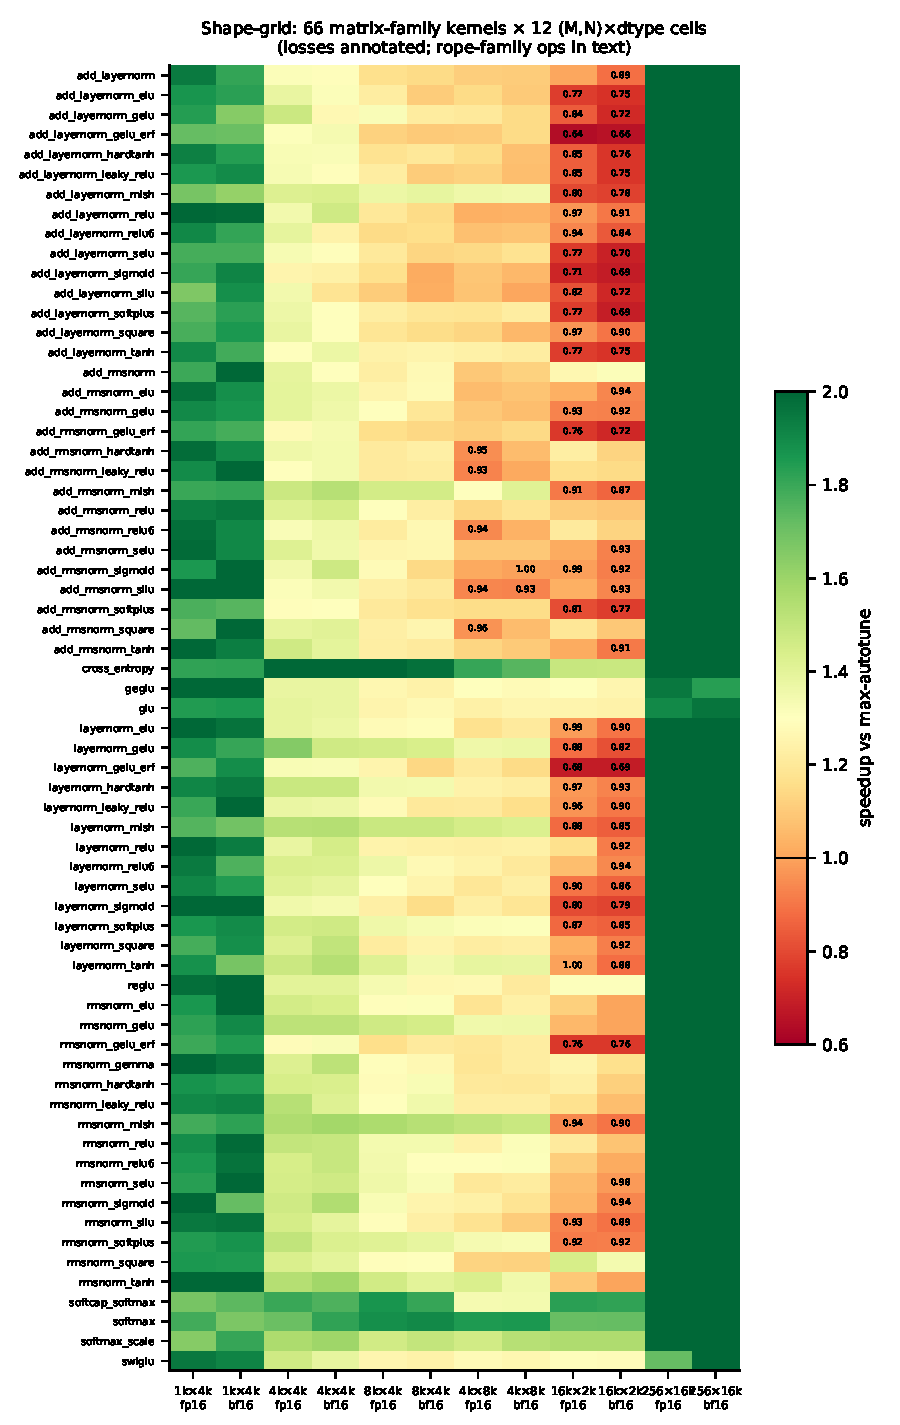
\includegraphics[width=0.78\textwidth]{figures/heatmap.pdf}
\caption{The shape grid. Green: beats \maxauto{} (recompiled per cell); annotated red
cells: losses, printed rather than hidden. The loss region is one regime, not noise.}
\label{fig:heatmap}
\end{figure}

\begin{figure}[t]
\centering
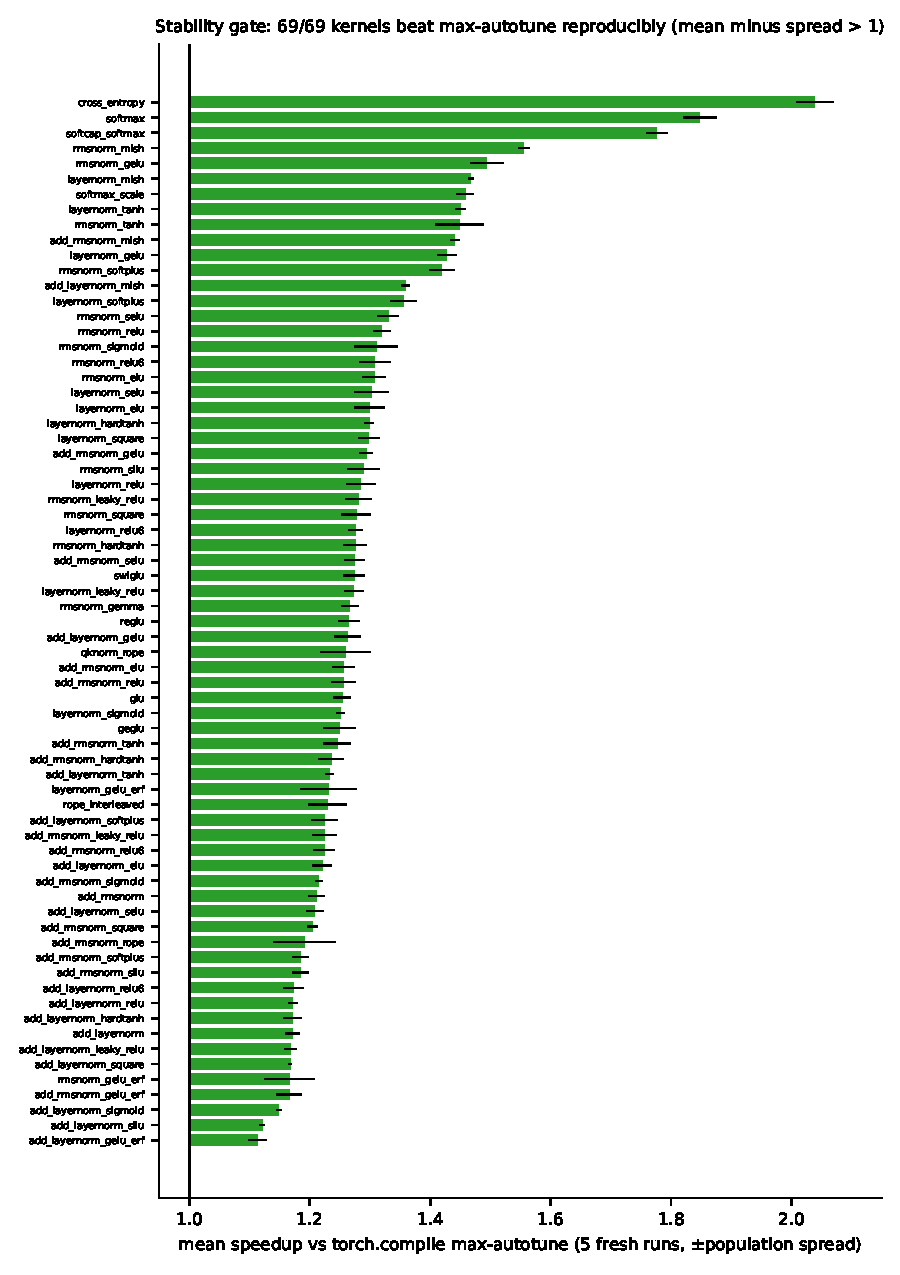
\includegraphics[width=0.8\textwidth]{figures/stability.pdf}
\caption{The $5\times$ stability gate over all \stabOps{} kernels: mean $\pm$ spread vs
\maxauto. Raw five-sample data for every bar ships in the repository.}
\label{fig:stability}
\end{figure}

\subsection{Against expert hand-written Triton: two conditions}\label{sec:experts}

Comparisons against Liger-Kernel, Unsloth, and the Triton tutorials run through the same
referee under two conditions: \emph{fixed-schedule} (raw extracted \texttt{@triton.jit}
kernels under our wrappers; schedule pinned) and \emph{library-API} (Liger called via its
own public \texttt{Function} interface, exactly as shipped). Ours is faster on
swiglu/rmsnorm/relu2/geglu in both conditions; softmax and layernorm are ties-within-noise
against the best fixed-schedule expert. Two honesty notes. First, \textbf{we retract our
own earlier claim} that 5 of 11 expert kernels were non-robust to odd shapes: under the
library-API condition all \hthApiVerified{} Liger recipes pass our adversarial sweep ---
the failures were artifacts of \emph{our} extraction wrappers. Second, the forward-only
cross-entropy comparison is \emph{unfair to Liger} (their CE computes gradients in the
forward by design) and is excluded from any headline.

\subsection{End-to-end composition}

A Qwen-style MLP block (add\_rmsnorm $\to$ gate/up GEMMs $\to$ swiglu $\to$ down GEMM)
runs three ways on identical weights; output verified against eager
(max err \eteErr) before timing. On H200 with trained kernels:
$\eteEagerX\times$ vs eager and $\eteCompileX\times$ vs whole-block compile-MA --- \emph{a
tie, reported as a tie}: GEMMs are \eteGemmFrac\% of the block and identical across paths,
bounding the achievable win (Amdahl) — though the non-GEMM sub-path itself is
$\eteNonGemmX\times$ faster. (On an RTX 4090 with gold seeds: $\eteEagerXLocal\times$ /
$\eteCompileXLocal\times$.) The single-op wins survive composition; they cannot and do not
claim block-level miracles.

\subsection{Teaching 37 unseen operators in one run}

Resuming the RL loop on 37 operators absent from all prior training (8 new epilogues
$\times$ norm/residual variants, plus softcap-softmax, Gemma-RMSNorm, GLU, interleaved
RoPE, fused cross-entropy), with the templated-mutation arm disabled (the model wrote
every candidate): \textbf{\vTwoOk/\vTwoOps{} validated correct and beat \maxauto{} on
fresh exit measurement} ($\vTwoMinMA\times$--$\vTwoMaxMA\times$), \vTwoLM/\vTwoOps{}
winning kernels model-authored, \vTwoVerified/\vTwoEvaluated{} sampled kernels verified
(\vTwoValidRate), \vTwoLeadTakes{} archive lead-takes, explore-arm contribution
\textbf{\vTwoExplore}. The model beat its own strongest gold seed on fused cross-entropy
($\vTwoCEMA\times$ vs \maxauto, model-authored). Learning is visible \emph{inside} the
run: the softplus/mish family --- which requires an overflow-guard idiom
($\mathrm{softplus}(x) = x$ for $x > 20$, else $\log(1{+}e^x)$) --- verified
\idiomPassOne{} per round on first encounter and \idiomPassTwo{} on the second pass,
after self-distillation on the first pass's verified winners (Fig.~\ref{fig:learning}).

\begin{figure}[t]
\centering
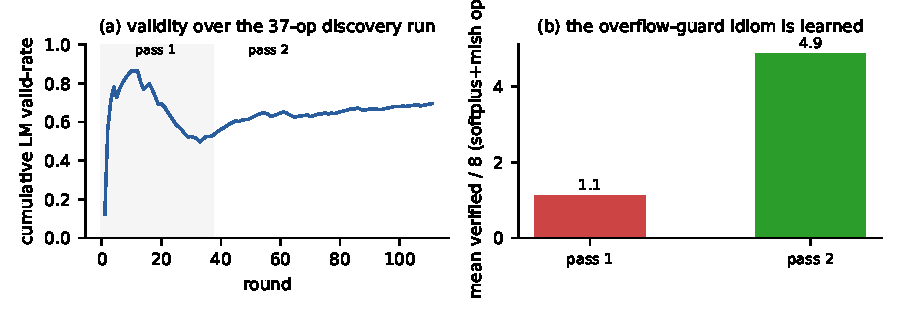
\includegraphics[width=0.85\textwidth]{figures/learning.pdf}
\caption{Learning where it matters: (a) cumulative validity over the 37-unseen-op run
dips as harder epilogue families arrive, then recovers as distilled idioms generalize;
(b) the overflow-guard idiom, quantified.}
\label{fig:learning}
\end{figure}

\subsection{The invention probe, and the repair of the loss regime}\label{sec:invention}

We then aimed the trained model at seven problems chosen to be \emph{foreign}:
\texttt{cumsum} (a prefix \emph{scan} --- carry propagation, a different parallel
algorithm class from every reduction in the suite), \texttt{entropy} and \texttt{kl\_div}
(coupled double reductions over logits), and four operators pinned to the
$16384\times2048$ loss regime identified by the shape grid. Pre-registered prediction
(ours, in writing): the regime requires split-row/multi-row schedules.

Outcome: \invOk/\invOps{} validated and beat \maxauto{}; \invLM/\invOps{} model-authored;
validity on foreign problems \invValidRate{} (vs $\sim$0.69 on familiar families --- an
honest difficulty gradient). Reading the kernels, not just the scores
(Fig.~\ref{fig:flip}):

\begin{itemize}
\item \textbf{The human diagnosis was wrong.} The winning kernels are plain
\emph{whole-row single-block} schedules; the losses were caused by looped templates tuned
at $N{=}4096$, not by row-per-program parallelism. The worst published loss cell
($\beforeALS\times$, \texttt{add\_layernorm\_sigmoid}) became a $\invALSshortMA\times$
win; \texttt{layernorm\_gelu} went $\beforeLG\times \to \invLGshortMA\times$;
softmax reached $\invSMshortMA\times$ in-regime.
\item \textbf{\texttt{cumsum} is invention-lite, labeled precisely.} The model did not
re-derive carry propagation; it recognized that a whole row fits one block and emitted a
loop-free \texttt{tl.cumsum} kernel --- beating our hand-written carry-loop gold by
$\sim$47\% ($\invCumsumMA\times$ vs \maxauto, $\invCumsumC\times$ vs compile), correct
across the full sweep. Primitive selection and schedule simplification, verified --- not a
new parallel algorithm.
\item \textbf{The capability boundary, stated:} on \texttt{entropy} and \texttt{kl\_div}
the model produced many verified kernels but never beat the hand-written two/three-pass
golds (which themselves stand at $\invEntropyMA\times$ and $\invKLMA\times$ vs \maxauto).
Authorship there remains human.
\end{itemize}

\begin{figure}[t]
\centering
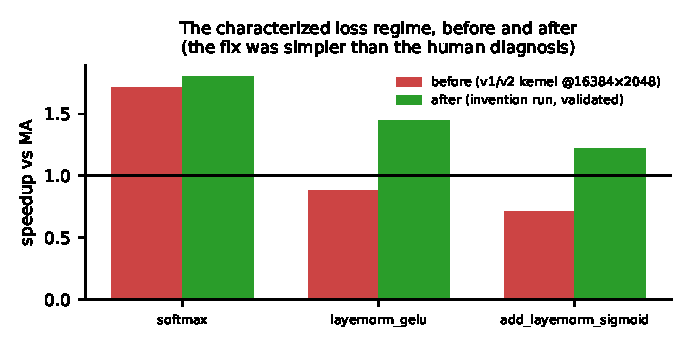
\includegraphics[width=0.6\textwidth]{figures/flip.pdf}
\caption{The characterized loss regime ($16384\times2048$, fp16), before and after the
invention run. The repair used a \emph{simpler} schedule family than the authors
predicted in writing.}
\label{fig:flip}
\end{figure}

\section{Ablations: where does the value come from?}\label{sec:ablations}

Four arms, identical except one ingredient (8 familiar ops, same SFT starting adapter,
24 rounds, group 8, single seed --- labeled): Table~\ref{tab:abl},
Fig.~\ref{fig:ablation}.

\begin{table}[t]
\centering\small
\begin{tabular}{lcccc}
\toprule
arm & removes & valid-rate & beat MA & geomean vs MA\\
\midrule
control & --- & \ablControlValid & \ablControlBeat & \ablControlGm\\
no-feedback & referee errors in prompt & \ablNofeedbackValid & \ablNofeedbackBeat & \ablNofeedbackGm\\
distill-only & policy-gradient term & \ablDistillonlyValid & \ablDistillonlyBeat & \textbf{\ablDistillonlyGm}\\
no-learn & all weight updates & \ablNolearnValid & \ablNolearnBeat & \ablNolearnGm\\
\bottomrule
\end{tabular}
\caption{Ablations on familiar operators (single seed; the ordering among
1.30--1.36 is suggestive, not established). The no-learn row's headline was recovered
from its completed report before a concurrent-write race overwrote the stored copy; the
race is documented and fixed in the artifact, and the arm's kernels remain archived for
re-validation.}\label{tab:abl}
\end{table}

\begin{figure}[t]
\centering
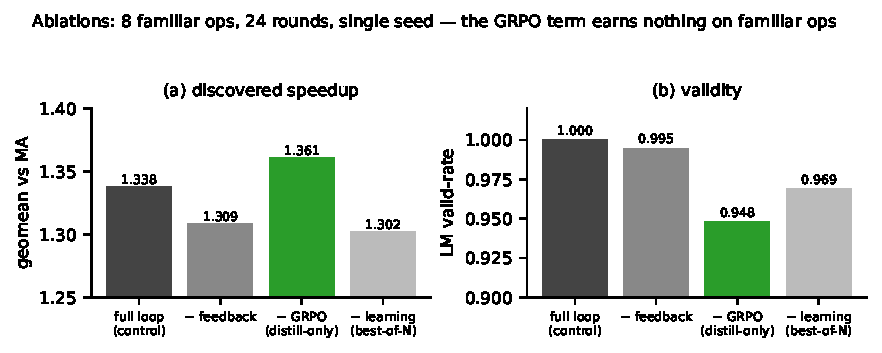
\includegraphics[width=0.8\textwidth]{figures/ablation.pdf}
\caption{Ablation arms. Removing the policy-gradient term does not hurt discovered
speedups on familiar ops; removing \emph{all} learning costs only a few percent there.}
\label{fig:ablation}
\end{figure}

Three observations, each contrary to at least one of our own pre-registered predictions:
\textbf{(1)} On familiar operators, the referee plus best-of-$N$ sampling from a frozen
competent model captures $\ablNolearnPctOfControl\%$ of the full loop's geomean ---
\emph{search, not learning, is the dominant force where competence exists}.
\textbf{(2)} The distill-only arm matched-or-beat control; the group-relative
policy-gradient term earned nothing here. Self-distillation on verified winners appears to
be the load-bearing learning ingredient. \textbf{(3)} Feedback's effect is unmeasurable at
the familiar-op validity ceiling --- its value, like learning's, concentrates on foreign
problems (the \invValidRate{} vs 0.69 validity gap and Fig.~\ref{fig:learning} are the
controlled contrast). A historical datum completes the picture: a 4.5-hour
\emph{continue-SFT} on new operators stalled and degraded proven operators and was
stopped, while RL-from-verifier taught the same operators cleanly --- corpus imitation is
not how the new capabilities arrived.

\section{The falsification ledger}\label{sec:falsification}

Because the referee is cheaper to consult than to argue with, we adopted the practice of
writing predictions down \emph{before} runs. Across the campaign the referee falsified
\falsifications{} confident human beliefs, including: the loss-regime diagnosis
(\S\ref{sec:invention}); the authors' hand-written scan kernel ($-47\%$); the published
expert-robustness claim (\S\ref{sec:experts}, retracted); the superiority of continue-SFT
for new operators; the ablation ranking (\S\ref{sec:ablations}); the adequacy of a subtle
anti-memoization perturbation (\S\ref{sec:antigaming} --- caught by the system's own
negative control); the verifiability of an innocuous-looking operator (\texttt{l1norm});
an early benchmark that manufactured compiler ties (\S\ref{sec:hygiene}d); and the
evidentiary value of all-green logs without durable artifacts (which forced a re-run of
our own stability gate under a written provenance note). We highlight this not as
housekeeping but as the paper's second thesis: \textbf{a system with an honest referee
does not require its builders to be right --- and will routinely demonstrate that they are
not.} The ledger, with open pre-registered predictions, ships in the artifact.

\section{Honest bounds}\label{sec:bounds}

(1) These are scheduling wins on bandwidth-bound fusion operators --- no claims against
cuBLAS/FlashAttention-class kernels, and no novel algorithm classes (the scan result is
primitive selection). (2) All speedups are vs \maxauto{} on specific hardware
(H200; spot-confirmed on RTX 4090); ratios are hardware-dependent even when reproducible.
(3) Ablations are single-seed and labeled. (4) KernelBench cross-evaluation is
out-of-scope-by-construction for our specialist (foreign format, generalist operators);
the recorded honest probe scored \kbCorrect/\kbN{} and we declined prompt-bridging
shortcuts that would manufacture a non-comparable number. (5) The loop requires a domain
with a cheap, un-gameable oracle and a measured quality signal; domains with judged
rewards are explicitly outside the recipe, and the framework's failure modes (expensive
oracles, adversarial environments, Goodhart on the metric) are discussed in the artifact.

\section{Reproducibility}

Everything regenerates from commands: the harness self-test
(\texttt{harness.py}; \selftestCasesHTwoHundred{} cases), the gates
(\texttt{rebench\_stability.py}, \texttt{rebench\_shapes.py}), training
(\texttt{modal\_app.py} entrypoints), and this paper's every number
(\texttt{paper/make\_numbers.py}, which fails the build on cross-report inconsistency)
and figure (\texttt{paper/make\_figures.py}). The artifact includes the
\productKernels{} kernels, adapters (2B and 27B), the verified corpus, raw five-sample
stability data, per-cell grid data, run transcripts where retrievable (with an honest
note on which are windows), and the falsification ledger.

\section{Conclusion}

\sys{} set out to show that the reward channel of an RL-for-code system can be hardened
the way security-critical code is hardened --- with its exploits implemented, committed,
and continuously rejected --- and that a commodity open model trained against such a
referee does real engineering: \productKernels{} reproducible compiler-beating kernels,
its own weak regime repaired, its builders corrected nine times. The model was swapped
once (2B$\to$27B) and could be swapped again; nothing in the result depends on its
identity. What cannot be swapped out is the referee. In domains where verification is
cheap and honest, that inversion --- \emph{the verifier is the asset; the model is a
commodity} --- is, we believe, the durable lesson, and the one most worth carrying to the
next domain.

\subsubsection*{Acknowledgments}
Engineering, experiments, and drafting were carried out with Claude (Anthropic) operating
the OUROBOROS pipeline end-to-end; all claims trace to harness-emitted artifacts rather
than to either human or model assertion. Compute: Modal (H200/L4) and a local RTX 4090.

\begin{thebibliography}{99}\small
\bibitem{sakana2025} Sakana AI. \emph{The AI CUDA Engineer}. Technical report and
subsequent public correction, February 2025.
\bibitem{kernelbench} A. Ouyang, S. Guo, et al. \emph{KernelBench: Can LLMs Write
Efficient GPU Kernels?} arXiv preprint, 2025.
\bibitem{kevin} C. Baronio, P. Marsella, et al. \emph{Kevin: Multi-Turn RL for Generating
CUDA Kernels}. arXiv preprint, 2025.
\bibitem{autotriton} S. Li et al. \emph{AutoTriton: Automatic Triton Programming with
Reinforcement Learning in LLMs}. arXiv preprint, 2025.
\bibitem{cudal1} X. Li et al. \emph{CUDA-L1: Improving CUDA Optimization via Contrastive
Reinforcement Learning}. arXiv preprint, 2025.
\bibitem{alphatensor} A. Fawzi et al. \emph{Discovering Faster Matrix Multiplication
Algorithms with Reinforcement Learning}. Nature 610, 2022.
\bibitem{alphadev} D. Mankowitz et al. \emph{Faster Sorting Algorithms Discovered Using
Deep Reinforcement Learning}. Nature 618, 2023.
\bibitem{stoke} E. Schkufza, R. Sharma, A. Aiken. \emph{Stochastic Superoptimization}.
ASPLOS, 2013.
\bibitem{deepseekmath} Z. Shao et al. \emph{DeepSeekMath: Pushing the Limits of
Mathematical Reasoning in Open Language Models}. arXiv:2402.03300, 2024.
\bibitem{tulu3} N. Lambert et al. \emph{T\"ulu 3: Pushing Frontiers in Open Language
Model Post-Training}. arXiv preprint, 2024.
\bibitem{pytorch2} J. Ansel et al. \emph{PyTorch 2: Faster Machine Learning Through
Dynamic Python Bytecode Transformation and Graph Compilation}. ASPLOS, 2024.
\bibitem{triton} P. Tillet, H.~T. Kung, D. Cox. \emph{Triton: An Intermediate Language
and Compiler for Tiled Neural Network Computations}. MAPL, 2019.
\bibitem{liger} P.-L. Hsu et al. \emph{Liger Kernel: Efficient Triton Kernels for LLM
Training}. arXiv preprint, 2024.
\end{thebibliography}

\end{document}
